\documentclass[12pt,a4paper]{article}
\usepackage[affil-it]{authblk}
\usepackage[utf8]{inputenc}

\usepackage{ragged2e}
\justifying

% Adjusting margins to personal my need
\addtolength{\oddsidemargin}{-.5in}
\addtolength{\evensidemargin}{-.5in}
\addtolength{\textwidth}{1in}
\addtolength{\topmargin}{-.5in}
\addtolength{\textheight}{1in}


% Graphics
\usepackage{caption}
\usepackage{graphicx}
\usepackage{subfigure}
\usepackage{float}
\graphicspath{{img/}}

% Math
\usepackage{amssymb}
\usepackage{amsmath} % Required for some math elements

% Other
\usepackage{algorithmic}
\usepackage{array}
\usepackage{lipsum}
\usepackage{hyperref}
\usepackage{multicol}

\renewcommand{\contentsname}{Indice}
\renewcommand\refname{Bibliografia}
\hypersetup{%
    pdfborder = {0 0 0}
}

\begin{document}
\title{Spambase\\
\Large{Report per l'Esame di Fondameti di Machine Learning}
} % Title

\author{\textsc{Marco Moroni} \\
    \emph{129056} \\
    Ingegneria informatica\\
    \emph{255699@studenti.unimore.it}
  }

\date{Giugno 2021}
\maketitle
\clearpage
\tableofcontents{}
\clearpage
\begin{abstract}
\normalsize
In questo progetto si andrà a trattare ed analizzare il problema delle email spam che oggigiorno è sempre più diffuso e nocivo, soprattutto per le grandi aziende. Grazie al dataset fornito e alle dovute analisi compiute su di esso si è riuscito a catalogare le email e predirre in modo pressochè perfetto la natura di una mail (veritiera o spam).
\end{abstract}

\clearpage
\section{Introduzione}
Con Spam si intende l’invio o la ricezione di messaggi pubblicitari di posta elettronica che non sono stati richiesti e che l’utente che li riceve non ha autorizzato il mittente ad inviare.
\hfill \break \break
Obiettivo degli spammer è la pubblicità: comuni offerte commerciali, proposte di vendita di materiale pornografico o illegale, farmaci senza prescrizione medica. Il loro scopo è quello di carpire dati personali, login e password di utenti, numeri di carte di credito e di conto corrente ecc…
\hfill \break \break
Gli spammer sono, a tutti gli effetti, dei criminali. Ad esempio quelli che inviano mail simili alla famosa truffa “alla nigeriana” dove una persona che non conosci ti chiede aiuto per sbloccare enormi  quantità di denaro e ti propone di dividere parte di quel denaro, ma ti chiede, per fare questa operazione, una serie di dati bancari che sono il vero e unico obiettivo della mail.
\hfill \break \break
Lo Spam è anche strumento di truffa, ti propone improbabili progetti finanziari, cerca di farti credere che hai fatto una favolosa vincita di denaro o sei stato designato erede di grandi fortune e per mandarti questo fiume di denaro chiede  le credenziali di accesso al tuo conto corrente online.
\hfill \break \break
Gli spammers inviano le mail pubblicitarie o truffaldine a migliaia di indirizzi, questi indirizzi sono raccolti in rete in molteplici modi:
\begin{itemize}
    \item automaticamente indirizzi mail da pagine personali, blog, forum o newsgroup;
\end{itemize}
\begin{itemize}
    \item usando appositi software che costruiscono gli indirizzi di mail usando nomi e cognomi comuni;
\end{itemize}
\begin{itemize}
    \item pubblicando falsi siti web che catturano indirizzi, promettendo vantaggi e offerte mirabolanti;
\end{itemize}
\begin{itemize}
    \item acquistando indirizzi mail da altri spammers.
\end{itemize}

Sorgono sempre più spesso notizie di grandi aziende, che per colpa di un dipendente non abbastanza istruito sul comportamento coretto da adottare di fronte ad una email non sicura, si ritrovano a dover sborsare migliaia di dollari da pagare in cryptovalute.

Motivo per il quale negli ultimi anni sempre più persone si stanno istruendo, e stanno istruendo gli altri sull'identificare 'a vista d'occhio' una mail spam, o comunque una mail sospetta.
\break
I vari servizi anti-spam che mettono a disposizione i diversi provider di mail (come Gmail, Outlook, Protonmail, Tutanota, Yahoo,...) il più delle volte non sono sufficienti a fermare i criminali che si nascondono dietro una banalissima ed innoqua email inviata dal 'cuggino di 4º grado con un patrimonio milionario bloccato alle isole mauritius'.

\clearpage
\section{Analisi dei dati}
In statistica, l'analisi esplorativa del dati (EDA - exploratory data analysis) è un approccio di analisi del set di dati per riassumere le loro caratteristiche principali, spesso usando grafici statistici e altri metodi di visualizzazione dei dati. Un modello statistico può essere usato o meno, ma principalmente l'EDA serve a vedere 'cosa i dati possono dirci'.L'EDA è diversa dall'analisi iniziale dei dati (IDA), che si concentra più strettamente sulla verifica delle ipotesi richieste per l'adattamento del modello e la verifica delle ipotesi, e sulla gestione dei valori mancanti e sulle trasformazioni delle variabili secondo necessità.

\subsection{Strumenti utilizzati}
Per questo lavoro ho trovato necessario l'utilizzo di alcune librerie open-source, fondamentali per l'analisi dei dati e per semplificare il lavoro dell'analista:
\begin{itemize}
    \item \textbf{pandas}: potente e veloce libreria nata per analizzare e manipolare i dati in input, il suo nome deriva dal gioco di parole "python data analysis";
\end{itemize}

\begin{itemize}
    \item \textbf{pyplot}: sottolibreria di matpolotlib che rende possibile la creazione di grafici, figure e linee, e permette inoltre di poter cambiare colori, forma e dimensioni.
\end{itemize}
\begin{itemize}
    \item \textbf{sklearn}: è una libreria di apprendimento automatico che contiene al suo interno algoritmi di ogni tipo;
\end{itemize}
\begin{itemize}
    \item \textbf{seaborn}: libreria basata su  matpolotlib, che come pyplot permette la creazione di grafici;
\end{itemize}

\begin{itemize}
    \item \textbf{numpy}: libreria basata su python e c++ fondamentale per lavorare con array di grandi dimensioni. A differenza delle liste di python, numpy salva i dati in memoria in maniera contigua, l'accesso, incrementando notevolmente le performance, stimate al 5000\%;
    \begin{figure}[h]
        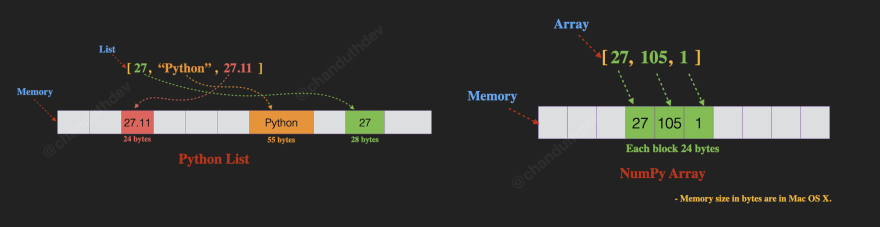
\includegraphics[width=1\linewidth]{numpy_vs_list.png}
        \caption{}
    \end{figure}

\end{itemize}

\clearpage
\subsection{Analisi inziale}
Per prima cosa è necessario capire con che tipo di dati si andrà a lavorare, che siano numeri interi o decimali, stringhe o booleani, è fondamentale saperlo prima di cominciare l'analisi.
Per fare ciò la libreria \textit{pandas} viene in supporto fornendo delle semplici funzioni ad-hoc, come\textbf{ \textit{pandas.info()}} che permette di ricavare il numero totale di righe e colonne, e per ogni attributo, specifica il tipo di dato della colonna.
\begin{figure}[h]
    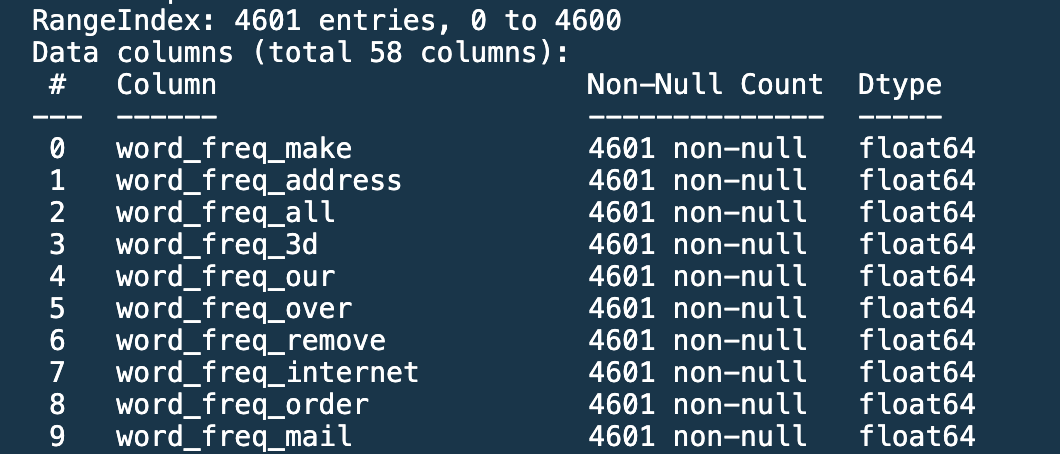
\includegraphics[width=1\columnwidth]{pandas_info.png}
    \caption{}
\end{figure}
Un'altra funzione utile è \textit{\textbf{pandas.describe()}} che per ogni colonna permette di ricavare dati come il numero di istanze non nulle, la media, la deviazione standard, il massimo e il minimo.

\begin{figure}[h]
    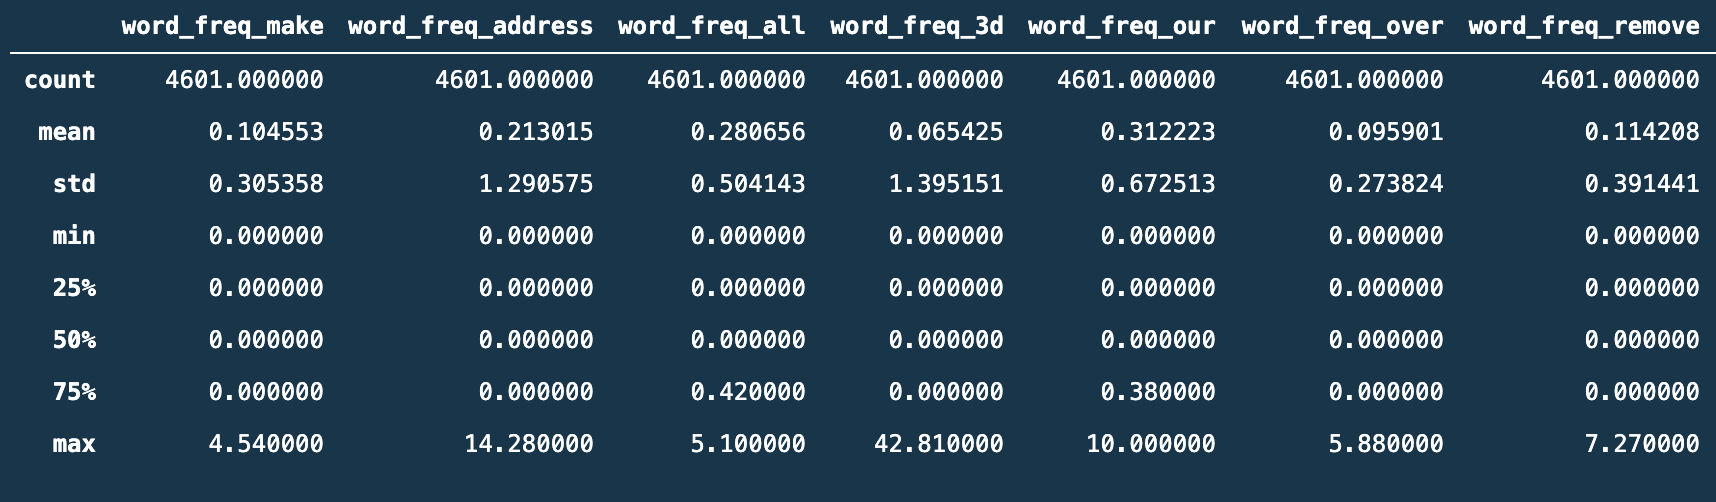
\includegraphics[width=1\columnwidth]{pandas_describe.png}
    \caption{}
\end{figure}
Il dataset è composto da 4601 istanze di email e 57 attributi rappresentati da un numero reale e un attributo classe rappresentato da un booleano che indica appunto se il sample è uno spam (1) o non spam (0).
Il dataset spambase in questione non è bilanciato, difatti le classi spam e non spam corrispondono rispettivamente al 39.4\% e 60.6\% dei samples raccolti.

\subsection{Correlazione}
La matrice di correlazione è una tabella che mostra come gli attributi  siano effettivamente legati tra loro. Quando due attributi sono tra di loro correlati, al crescere dell’uno cresce anche l’altro.

Il coefficiente di correlazione è un numero, compreso tra -1 e + 1 che esprime il grado di dipendenza tra due attributi, ed in base al valore che assume si può dedurre che se il coefficente è:

\begin{itemize}
\item == 1: i due attributi hanno la stessa curva, al crescere dell'uno cresce anche l'altro;
\item == -1: i due attributi sono perfettamente decorrelati con una curva inversamente proporzionale, al crescere del primo il secondo decresce;
\item == 0: i due attributi sono indipendenti l'uno dall'altro.
\end{itemize}
 Si può notare dal grafico in figura 4 che la diagonale è composta da tutti 1, dato che un attributo messo in relazione con se stesso seguirà la stessa curva.
\begin{figure}[H]
    \centering
    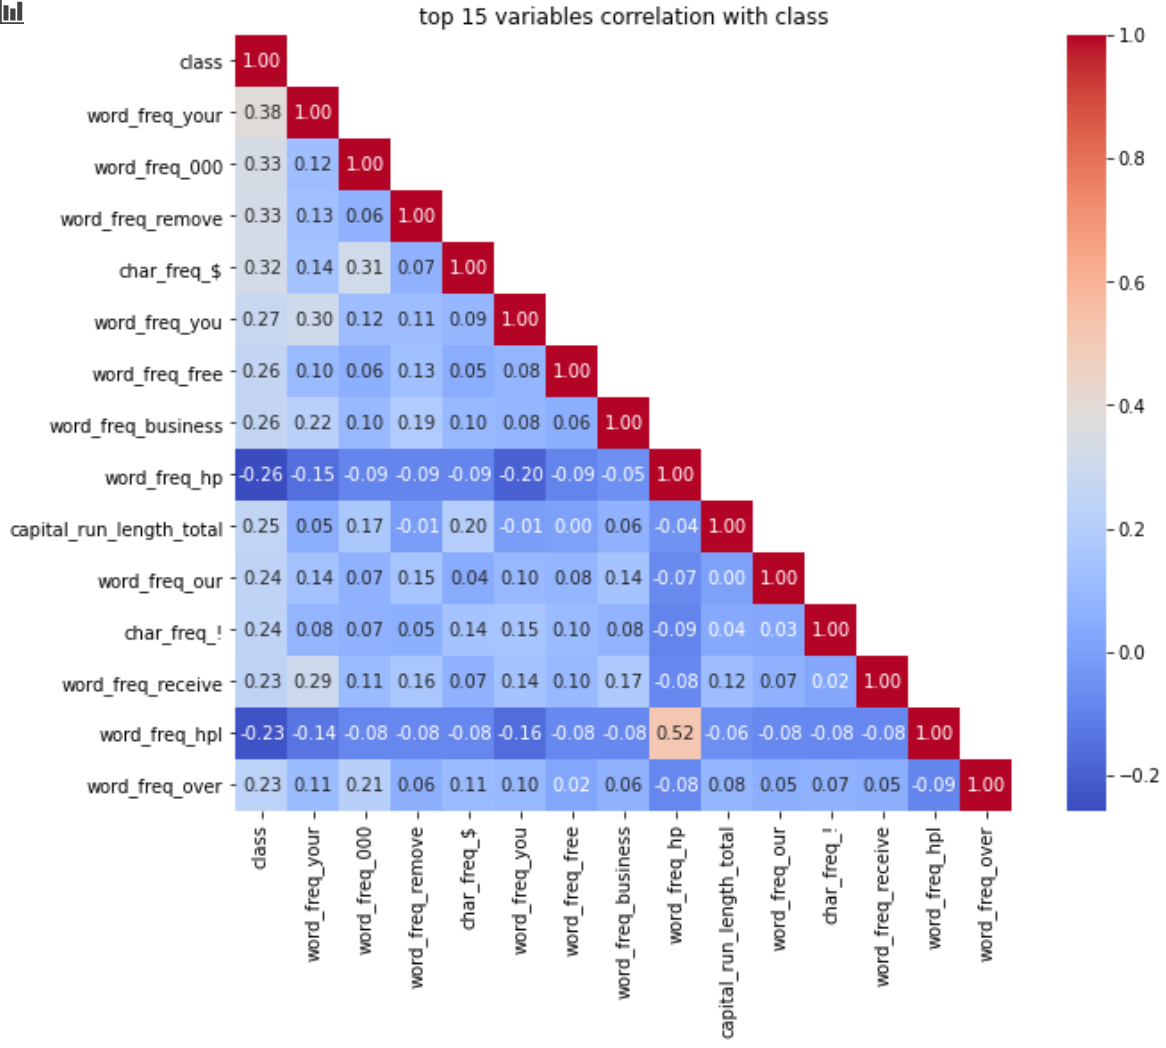
\includegraphics[scale=0.5]{correlation_top_15.png}
    \caption{}
\end{figure}
Il grafico di correlazione riesce a mettere in evidenza gli attributi più collegati con la classe (spam o non spam). In ordine, si notano le parole "your", "0000", "remove", "\$", "you", "free", "business", "hp", "capital\_run\_lenght\_total" (numero di lettere maiuscole), "our", "!", "receive", "hpl", "over".

Raffigurati ci sono i primi 15 attributi più collegati alla classe spam, anche se non si nota una stretta coerelazione, dato che i valori si muovono tra 0.23 e 0.38.

Si va quindi a restringere il campo per analizzare, sempre graficamente, la corrispondenza tra i cinque attributi più correlati. Si denota facilmente, dalla figura 5, che la parola "your" è più presente nelle email non spam, mentre le parole "000", "remove", "\$" e "you" sono nettamente più frequenti nelle email spam.

\begin{figure}[H]
    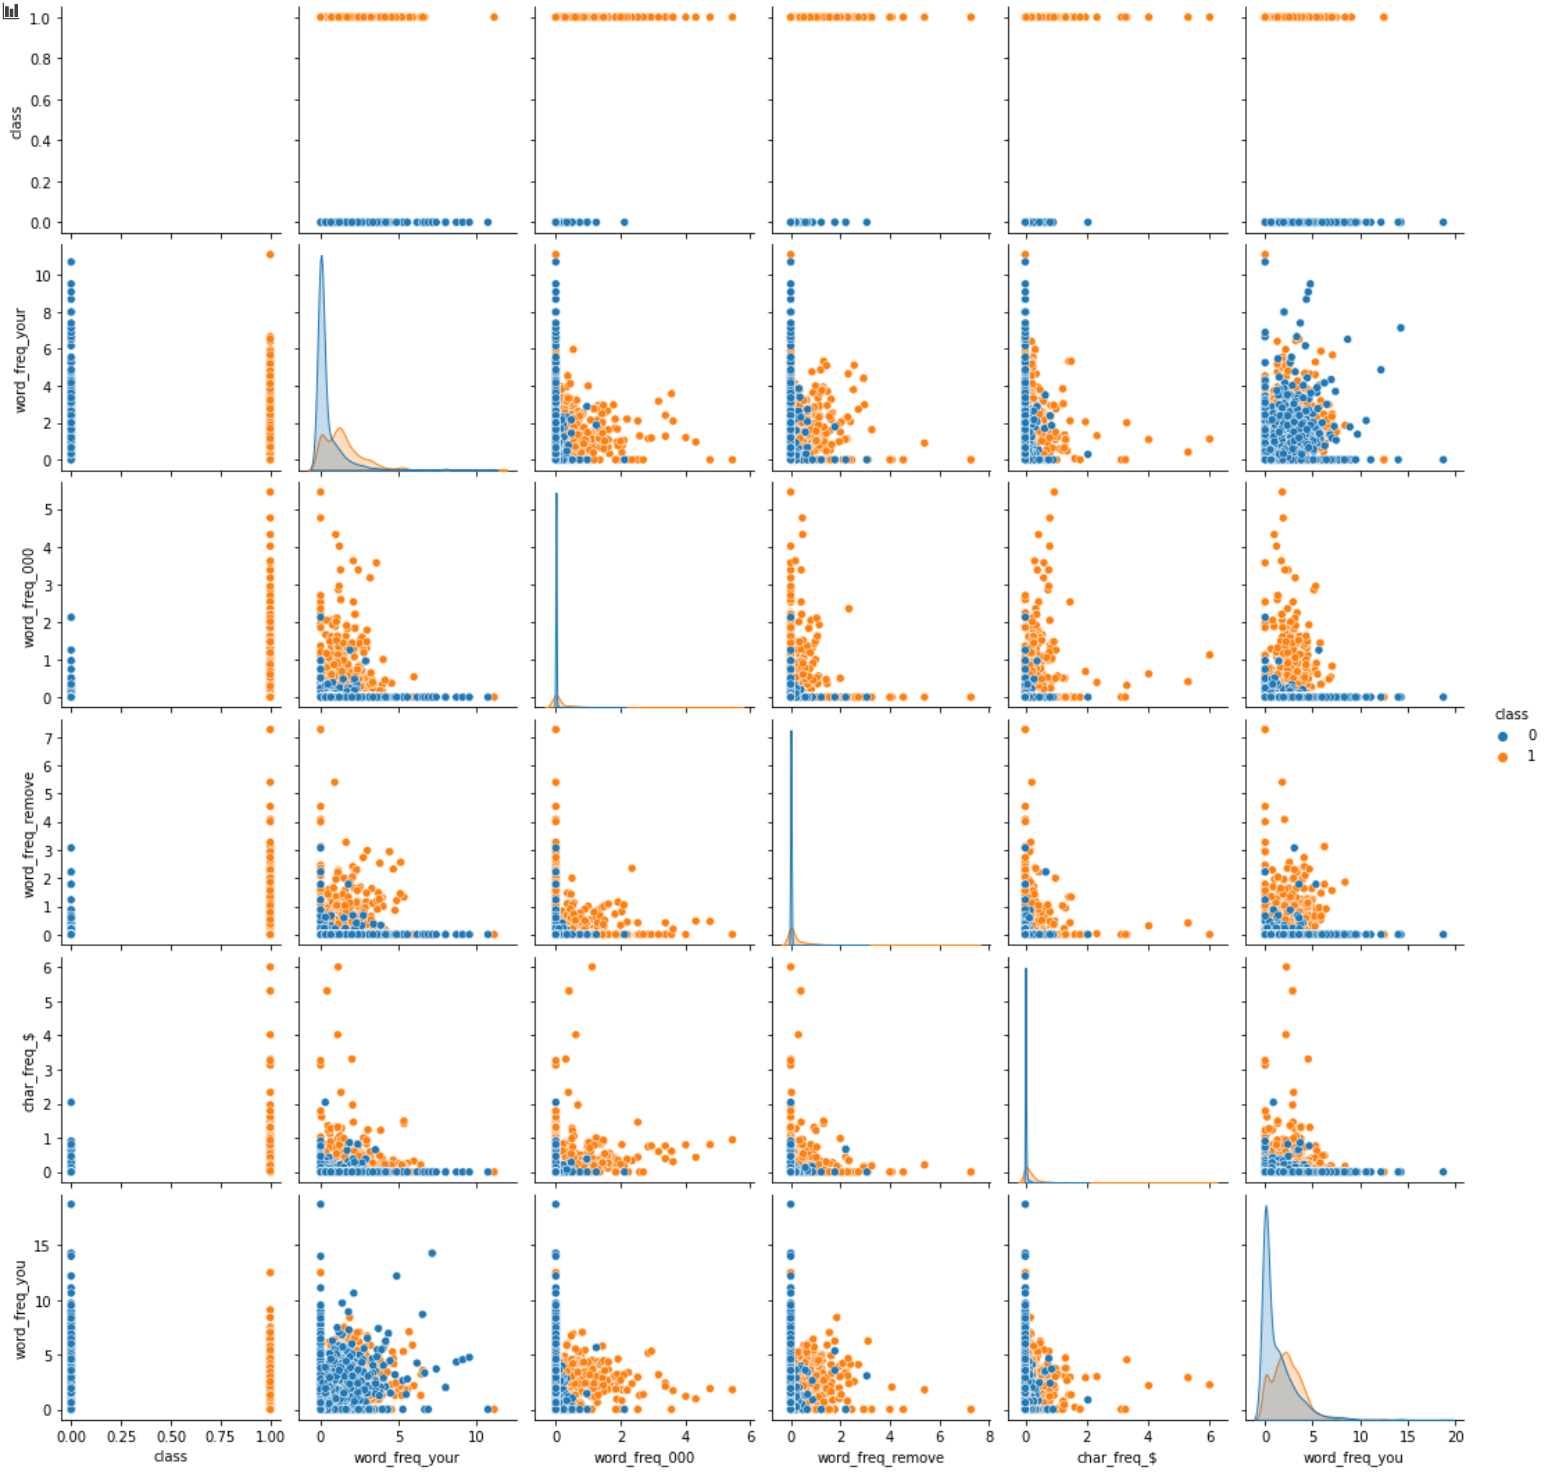
\includegraphics[width=1\columnwidth]{correlation_pair_top_6.png}
    \caption{}
\end{figure}
\clearpage
\subsection{Comparazione parole}
In questa sezione si andranno ad analizzare quali saranno le parole effettive da tenere maggiormente in considerazione tramite 3 grafici esplicativi.


Il grafico in figura 6 rappresenta la percentuale della frequenza di ogni singola parola trovata nelle email che sono state poi selezionate come spam. In questo grafico non si tiene conto dell'influenza delle email non spam. Il grafico conferma le analisi svolte nei capitoli precedenti, questa volta calcolando solo l'impatto delle email non spam. Le due parole più inserite sono sempre "you" e "your".


\begin{figure}[H]
    \centering
    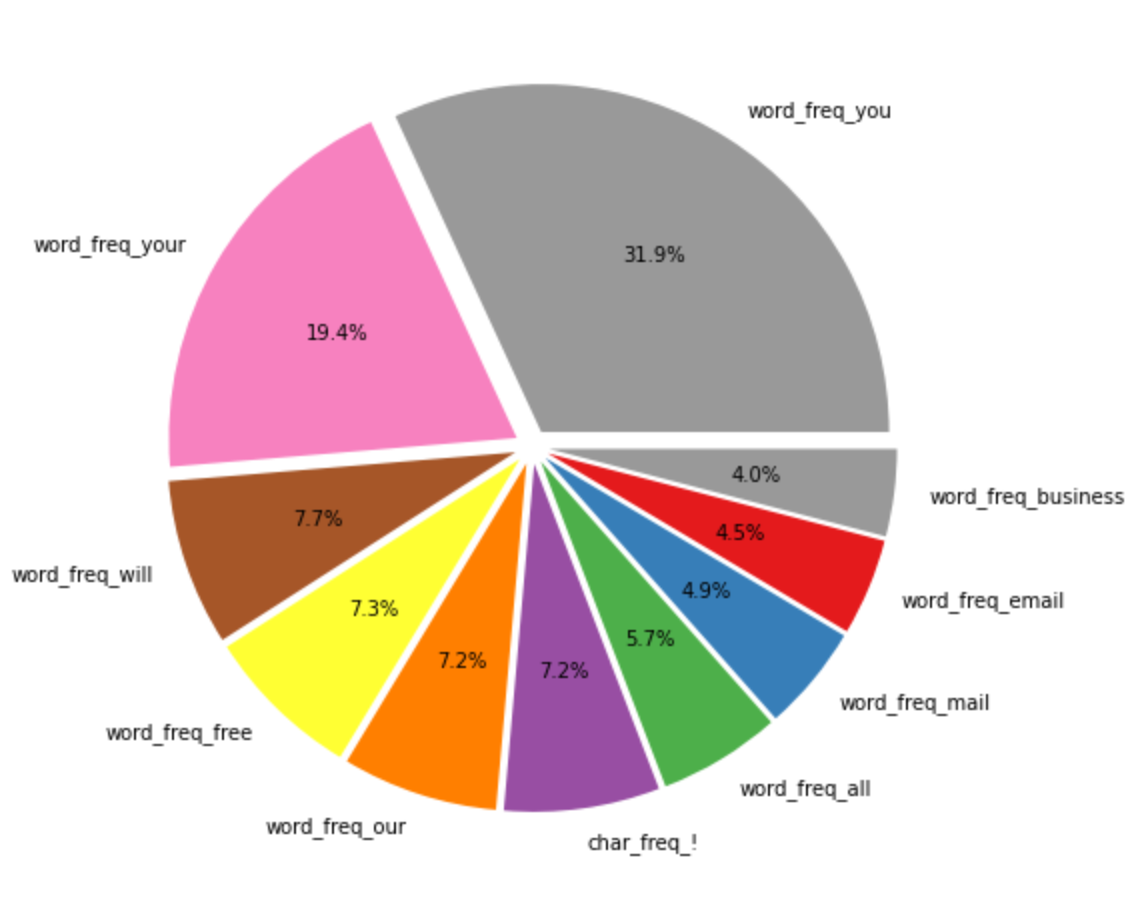
\includegraphics[width=.8\linewidth]{top_10_only_spam.png}
    \caption{}
\end{figure}
Per eseguire un'analisi più scrupolosa si va invece a calcolare la differenza delle frequenze tra le email non spam e le email spam.
Per fare ciò è prima necessario creare una tabella pivot che calcoli, per entrambe le classi, la media di attributo, restituendo una tabella (figura 7) che abbia sulle ascisse le parole chiave e sulle ordinate la classe di appartenenza; i valori corrispondenti saranno la media delle frequenze della parola X nella rispettiva classe di appartenenza Y.
\begin{figure}[H]
    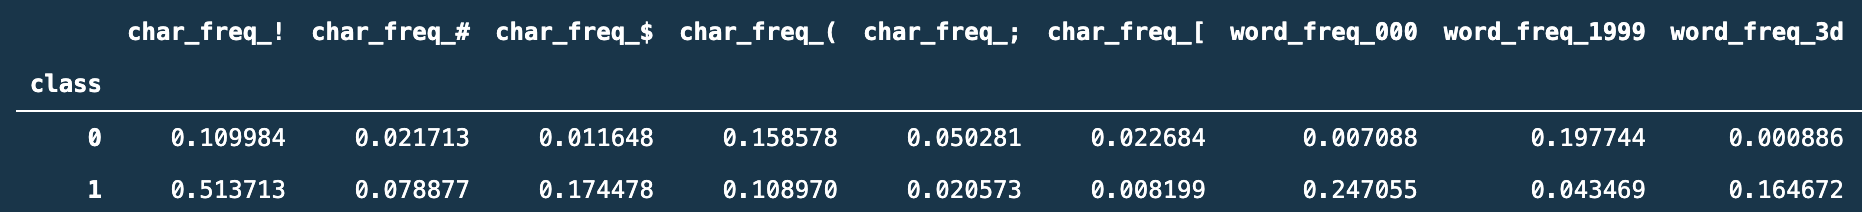
\includegraphics[width=1\linewidth]{pivot.png}
    \caption{}
\end{figure}
Una volta calcolata la tabella pivot si notano immediatamente, dal grafico in figura 8, le parole che hanno un maggiore impatto sulla scelta della classe di appartenenza. In base al valore che ogni barra assume sulle y si determina che se:
\begin{itemize}
    \item y == 0: la parola è equamente presente sia nelle email spam che non spam;
    \item y \textless  \! 0: la parola è maggiormente presente nelle email spam;
    \item y \textgreater \!  0: la parola è maggiormente presente nelle email non spam.
\end{itemize}

\begin{figure}[H]
    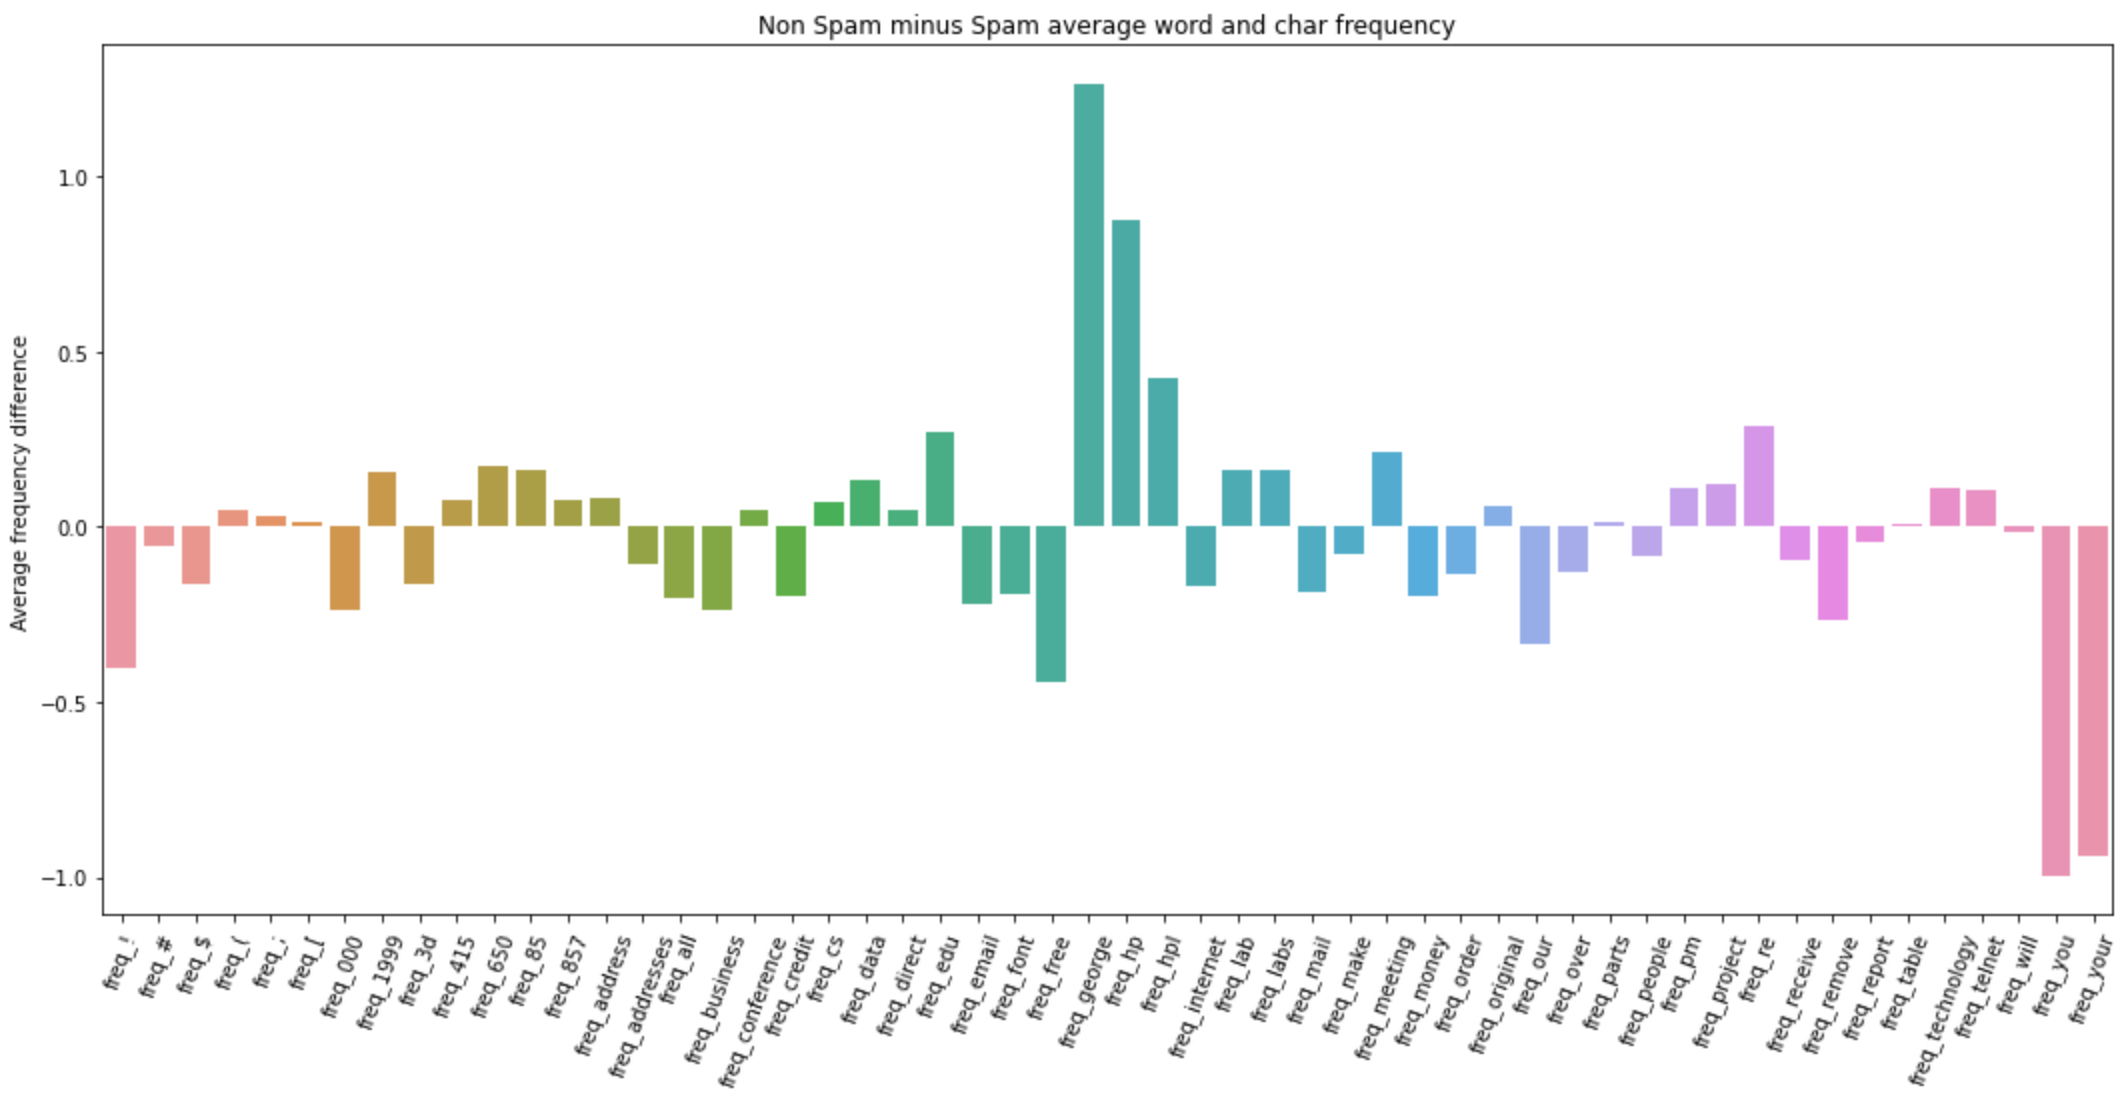
\includegraphics[width=1\columnwidth]{df_difference_barplot.png}
    \caption{}
\end{figure}

Spiccano all'occhio, quindi, che le parole "you" e "your" sono nettamente più frequenti nelle email spam, mentre le parole come "george" e "hp" sono maggiormente più frequenti nelle email vere. Questo perchè spesso, il malintenzionato che spedisce la mail malevola, non conosce il nome delle proprie vittime e si rivolge a loro con il pronome "you" ("tu", in inglese), piuttosto che con il loro vero nome.
\subsection{Lettere maiuscole}
Nel dataset, oltre alla frequenza delle singole parole, sono presenti tre campi aggiuntivi:
\begin{itemize}
    \item capital\_run\_lenght\_average: indica la media delle lunghezze di ininterrote sequenze di lettere maiuscole;
    \item capital\_run\_length\_longest: indica la sequenza di lettere maiuscole più lunga;
    \item capital\_run\_length\_total: indica la somma totale delle lettere maiuscole.
\end{itemize}

Analizzando questi tre fattori presenti all'interno della email, si deduce, leggendo il grafico a figura 9 con le stesse valutazioni del grafico a figura 8, che nelle email spam è nettamente maggiore il numero di lettere maiuscole inserite, che nelle email non spam.
Il malintenzionato preferisce, quindi, utilizzare le lettere maiuscole per carpire l'attenzione della vittima.

\begin{figure}[H]
    \centering
    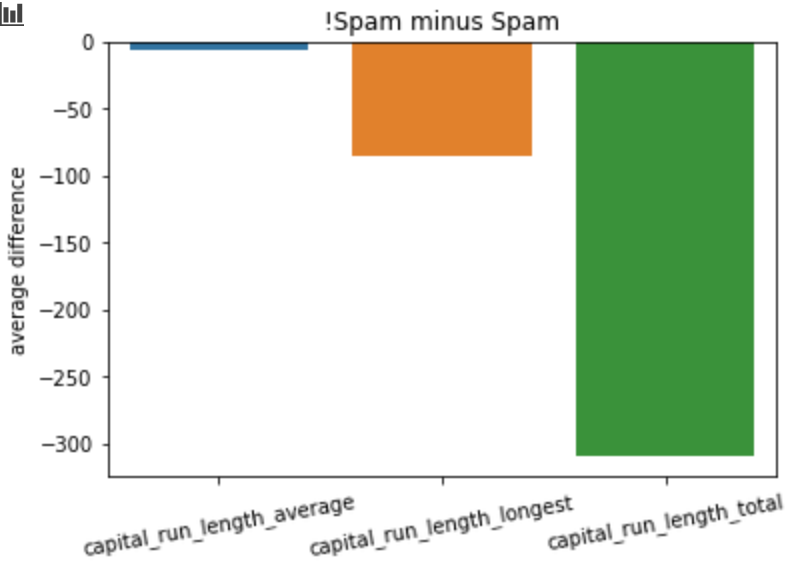
\includegraphics[width=.9\columnwidth]{capital_plot.png}
    \caption{}
\end{figure}
\clearpage
\section{Discussione dei modelli}
In questo capitolo si andranno ad analizzare gli algoritmi utilizzati per prevedere la  natura di una mail.

Il problema in questione fa chiaramente riferimento ad un modello di classificazione binaria, poichè ogni sample è rappresentato da un numero intero e può assumere solamente due valori:
\begin{itemize}
    \item 0: non spam;
    \item 1: spam.
\end{itemize}
Per questo progetto ho selezionato, tra gli algoritmi svolti durante le lezioni, tre che ho reputato più adatti per il riconoscimento, che si andranno ad esaminare più approfonditamente nelle prossime sezioni:
\begin{itemize}
    \item K-Nearest Neighbors;
    \item Alberi decisionali;
    \item Support Vector Machine (SVM)
\end{itemize}

\clearpage
\subsection{K-Nearest Neighbors}
K-Nearest Neighbors è un algoritmo che si basa sulle caratteristiche dei K-vicini (dove K è un numero intero positivo che indica il numero di vicini da prendere in considerazione) per determinare la classe di appartenenza di ogni sample.
In questo tipo di classificazione, il risultato è l'appartenenza ad una certa classe.

\begin{figure}[h]
    \centering
    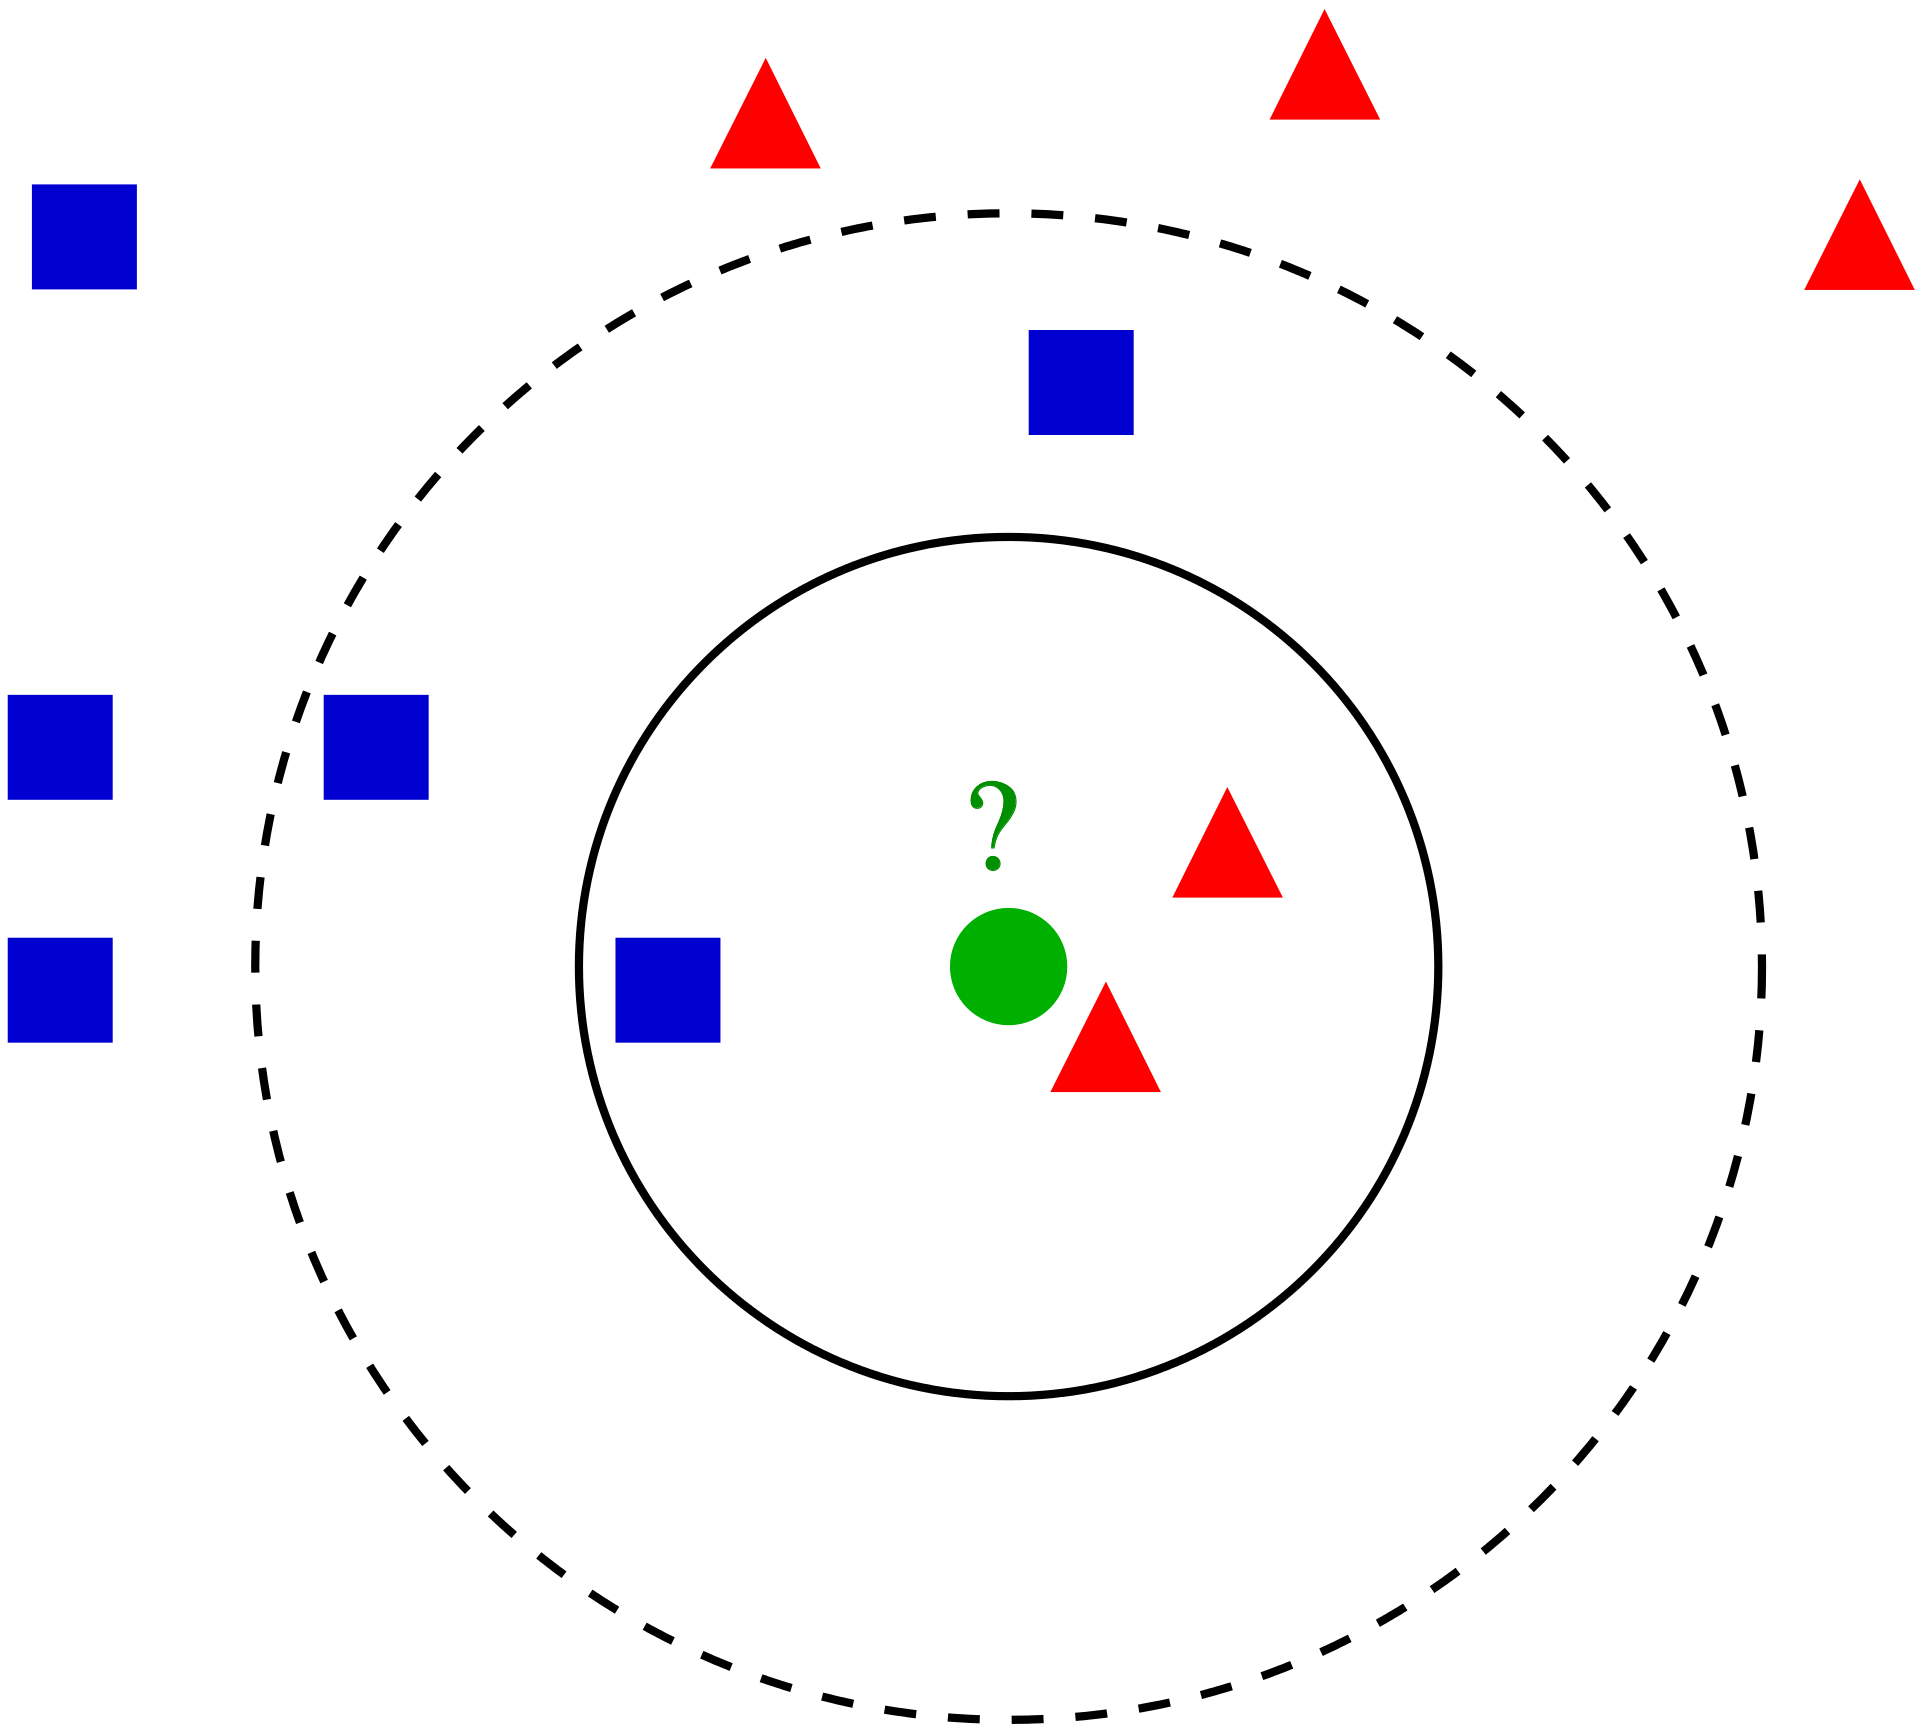
\includegraphics[scale=0.07]{KnnClassification.png}
    \caption{}
\end{figure}

Questo algoritmo, quindi descrive la similarità tra i diversi sample, in base al numero di vicini che vengono presi in considerazione. Per esempio, per prevedere la classe della pallina verde in figura 10 la scelta di un k diverso cambia il risultato:
\begin{itemize}
    \item k == 3: si considerano i tre oggetti più vicini e si tiene conto del maggiore, 2 triangoli rossi e 1 quadrato blu, quindi la pallina verde viene associata alla stessa classe dei triangoli rossi, in quanto numero maggiore dei quadrati blu;
    \item k == 5: ragionamento analogo, si contano 3 quadrati blu e 2 triangoli rossi, la pallina verde viene quindi associata alla stessa classe dei quadrati blu.
\end{itemize}

La scelta del valore k può quindi rovesciare la previsione dell'intero algoritmo. Solitamente k è un numero non molto grande, e per una classificazione binaria è preferibile un k dispari, per evitare di ritrovarsi in situazioni di parità (3 quadrati blu e 3 triangoli rossi). \hfill \break

Questo tipo di algoritmo è molto influenzato dall'uniformità dei dati ed il dataset preso in considerazione non è bilanciato (60\% non spam e 40\% spam), per ciò per il seguente algoritmo i parametri scelti per ottimizzare al massimo l'algoritmo sono stati:
\begin{itemize}
    \item \textbf{weight} = "distance": nell'esempio di prima dei triangoli, ogni elemento aveva lo stesso peso nella conta; utilizzando questo parametro, gli elementi più vicni alla pallina verde avranno un peso maggiore, mentre quelli più distanti avranno un peso minore;
    \item \textbf{k = 14}: nonostante si tratti di una classificazione binaria, utilizzando la distanza pesata, perde di senso utilizzare per forza un numero dispari per evitare di imbattersi in condizioni di parità.
\end{itemize}

\subsection{Alberi  decisionali}
Con alberi decisionali s'intende l'implementazione degli alberi binari, composti da:
\begin{itemize}
    \item \textbf{nodi}: funzioni condizionali booleane che testano il valore dello specifico attributo;
    \item \textbf{rami}: collegamenti tra i nodi, rappresentano il risultato della condizione;
    \item \textbf{foglie}: una sottoclasse dei nodi, rappresentano il risultato finale della previsione di classificazione.
\end{itemize}

\begin{figure}[h]
    \centering
    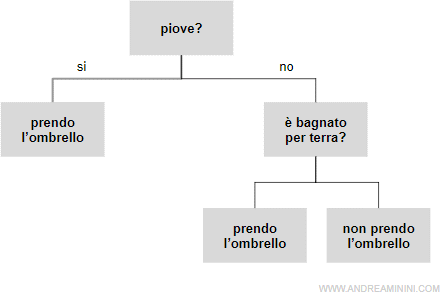
\includegraphics[width=.5\columnwidth]{decision_tree.png}
    \caption{}
\end{figure}
Una regola di suddivione è necessaria per decidere quale (o quali) variabile deve essere utilizzata nella condizione di un nodo per dividere il set di dati in sttogruppi, e soprattutto quale soglia utilizzare sulle variabili. Il metodo con cui vengono effettuate queste suddivisioni è basato sull'impurità dei nodi.

Si definisce "nodo impuro" un nodo che ha come risultato più classi diverse, mentre un "nodo puro" è un nodo che ha una sola classe come risultato.
L'impurità in un nodo è quindi:
\begin{itemize}
    \item \textbf{massima} quando tutte le classi nel nodo (in questo caso due) sono presenti in maniera casuale;
    \item \textbf{minima} quando nel nodo è presente una sola classe di appartenenza.
\end{itemize}
L'indice di Gini e l'entropia sono due criteri per calcolare l'impurità di un nodo, quindi la probabilità che una particolare variabile sia classificata in modo errato quando scelta casualmente.

Per il seguente algoritmo i parametri scelti per ottimizzare al massimo l'algoritmo sono stati:
\begin{itemize}
    \item \textbf{l'indice di}\textbf{ Gini}: varia tra 0 e 1, come si è discusso precedentemente, quando il valore è massimo (1) gli elementi son distribuiti casualmente nelle classi, minimo (0) quando tutti gli elementi appartengono alla stessa classe, e medio (0.5) quando gli elementi sono equamente distribuiti tra le due classi;
    \item \textbf{profondità massima = 10}: cioè la il numero massimo di livelli che ci possono essere nella rappresentazione dell'albero (per esempio, nella figura 11, sono presenti 3 livelli, compreso il nodo radice).
\end{itemize}

Di default non c'è un limite alla profondità massima che un albero può raggiungere, ma così facendo, si rende la previsione soggetta ad \textit{overfitting}.

L'\textit{overfitting} è una condizione nella quale il modello creato si adatta perfettamente ai sample con cui ha eseguito "l'allenamento" cioè con quali istanze di email ha creato l'albero; ma non riesce poi ad adattarsi nello stesso modo con nuovi sample.
Di norma, più si incrementa il numero massimo di profondità, più l'albero diventa complesso e più specifico a determinate condizioni, di conseguenza meno flessibile ed adattabile, soggetto quindi ad overfitting.

Può verificarsi anche la situazione opposta dove si imposta un numero massimo di livelli troppo basso, così da non lasciare possibilità al modello di creare le condizioni minime per classificare i sample e generalizzando troppo il risultato. Questa condizione specifica prende il nome di \textit{underfitting}.

\subsection{Support Vector Machine}
Le macchine a vettori di supporto sono dei modelli di apprendimento supervisionato con l'obiettivo di identificare l'iperpiano linerare che meglio divide i sample in classi. In caso di classificazione con due sole dimensioni spaziali (x, y) l'iperpiano si riduce ad una riga, mentre a tre dimensioni viene rappresentato da un piano a tutti gli effetti, invece con più di tre dimensioni viene appunto definito \textit{iperpiano}.

Si definiscono
\begin{itemize}
    \item vettori di supporto: i punti più vicini all'iperpiano;
    \item margine: distanza tra i due vettori di supporto (di due classi differenti) più vicini all'iperpiano.
\end{itemize}

\begin{figure}[H]
    \centering
    \subfigure[]{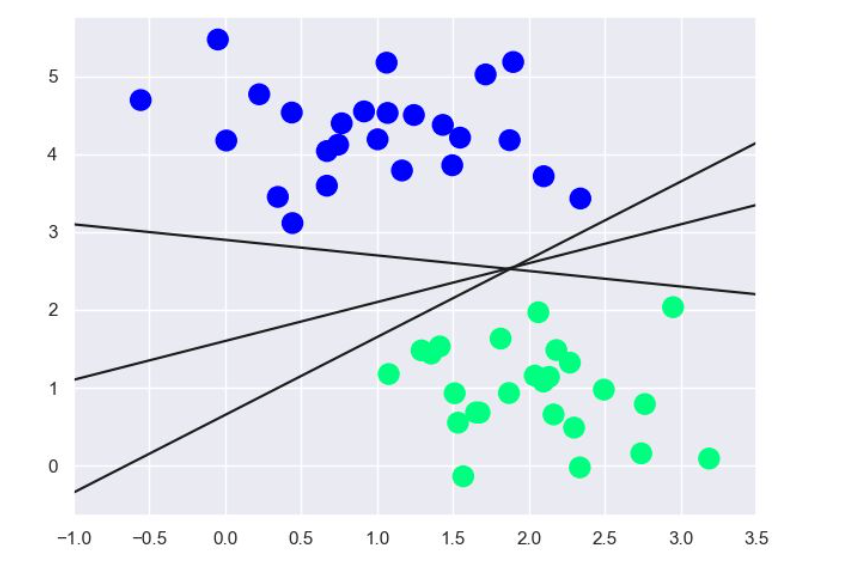
\includegraphics[width=0.48\linewidth]{svc.png}}
    \subfigure[]{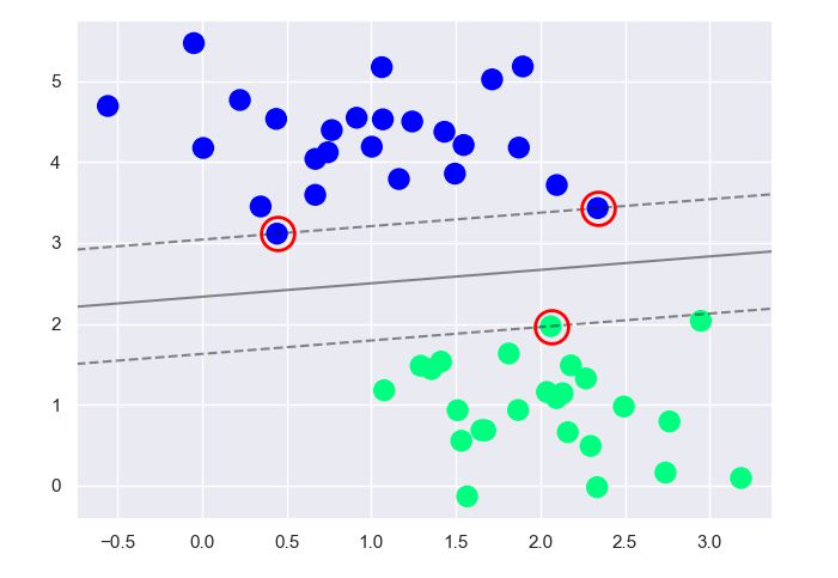
\includegraphics[width=0.48\linewidth]{svc_margin.png}}
    \caption{}
\end{figure}



L'algoritmo quindi disegna un numero n di linee per separare le palline blu da quelle verdi e calcola quale tra queste risulta ottimale per la separazione delle due classi.

\begin{multicols}{2}[\columnsep2em]
    Per modelli più complessi è necessario poter utilizzare, oltre che a linee rette, anche curve e regioni complesse nello spazio.
    Questo viene fatto attraverso un \textit{kernel}, cioè una funzione che sposta i dati da un piano a bassa dimensione in uno spazio e dimensione superiore dove è possibile separarli tramite un piano.

    Per questo algoritmo si è scelto di utilizzare un kernel \textbf{RBF} (radial basis function) che permette di creare regioni complesse nello spazio delle features.
    \columnbreak

    \begin{figure}[H]
        \centering
        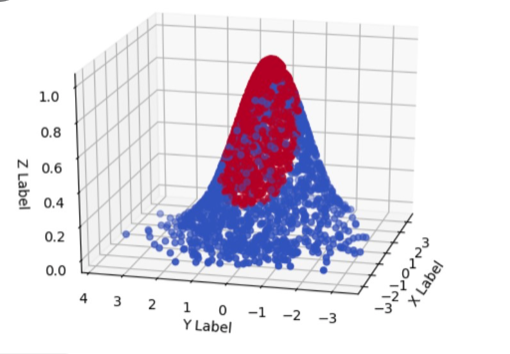
\includegraphics[width=1\linewidth]{rbf.png}
        \caption{}
        \label{fig:my_label}
    \end{figure}
\end{multicols}


\subsection{Ensamble}

Con \textit{ensamble} s'intende l'utilizzo modelli multipli per ottenere una migliore prestazione predittiva rispetto ai modelli singoli da cui è costituito. Ogni modello effettua la predizione della classe di appartenenza, e successivamente viene considerata valida la predizione fatta dal maggior numero di essi.
Esistono tre tecniche differenti di ensamble:
\begin{itemize}
    \item \textbf{bagging}: questa tecnica mira a creare un insieme di classificatori aventi la stessa importanza. All'atto della classificazione, ciascun modello voterà circa l'esito della predizione e l'output complessivo sarà la classe che avrà ricevuto il maggior numero di voti;
    \item \textbf{boosting}: a differenza del bagging, ciascun classificatore influisce sulla votazione finale con un certo peso. Tale peso sarà calcolato in base all'errore di accuratezza che ciascun modello commetterà in fase di learning;
    \item \textbf{stacking}: mentre nel bagging l'output era il risultato di una votazione, questa tecnica consente a un algoritmo di addestramento di raggruppare diverse altre previsioni di algoritmi di apprendimento simili.
\end{itemize}

Ho applicato questa la tecnica dell'ensamble all'algoritmo con i risultati migliori: gli alberi decisionali.
L'algoritmo di ensamble degli alberi decisionali viene denominato \textbf{Random Forest}, che è un estensione del bagging. Questo algoritmo prende in esame n alberi diversi e, oltre a prendere un sottocampione diverso di dati per ogni albero, estrae anche le caratterstiche (attributi) in modo casuale, piuttosto che usare sempre tutte le caratteristiche per fare "crescere gli alberi".\hfill\break
L'algoritmo prende quindi il nome di Random Forest (Foresta casuale) dato che si hanno molteplici alberi casuali.

Utilizzando questa tecnica sull'algoritmo migliore, la previsione è incrementata di circa l'1\%.

\subsection{Scelta indicatori}
Per l'analisi delle prestazioni di un algoritmo è necessario tener conto degli indicatori in base a diversi fattori, sia al tipo di classificazione che al dataset.
Gli indicatori classici che solitamente si vanno ad osservare sono:
\begin{itemize}
    \item \textbf{accuracy}: indica il rapporto tra i valori corretti (sia positivi che negativi) sul totale dei sample
    \begin{equation}
         accuracy = \frac{ TP+TN}{TP+FP+FN+TN}
    \end{equation}

    \item \textbf{precision}: indica il rapporto tra le osservazioni positive correttamente predette e il totale delle osservazioni positive predette
    \begin{equation}
         precision = \frac{ TP}{TP+FP}
    \end{equation}

    \item \textbf{recall}: indica il rapporto tra le osservazioni positive correttamente predette e tutte le osservazioni effettive della classe
    \begin{equation}
         recall = \frac{TP}{TP+FN}
    \end{equation}

    \item \textbf{f1 score}: indica la media ponderata tra precision e recall e prende quindi in considerazione sia i falsi positivi che i falsi negativi
    \begin{equation}
         f1\_score = \frac{2*Recall * Precision}{Recall + Precision}
    \end{equation}
\end{itemize}
In una classificazione binaria, come in questo caso, quando il dataset non è uniforme, cioè il numero di sample delle due classi non è simile ma si discosta di molto l'uno dall'altro come in questo caso (60\% non spam, 40\% spam) è necessario fare delle osservazioni.

Utilizzare l'accuracy sarebbe non totalmente corretto, perchè questo indice di misurazione è preciso solo se si sta lavorando con un dataset bilanciato (non è il caso in considerazione);
eventualmente si potrebbe utilizzare l'\textit{accuracy per classe} che va ad indicare l'accuratezza della previsione per ogni classe.

Per questo progetto si è scelto di utilizzare come indice l'\textbf{f1-score}, che da una rappresentazione più reale e corretta dei dati in questione. L'f1-score prende in considerazione sia i falsi negativi che i falsi positivi ed è meno intuitivo da interpretare, ma molto più adatto dell'accuracy quando il dataset non è uniforme.

Di seguito vegono riportate le \textit{confusion matrix} per ogni algoritmo, che vanno a rappresentare graficamente il risultato di ogni classificatore binario.


\begin{figure}[H]
    \centering
    \subfigure[]{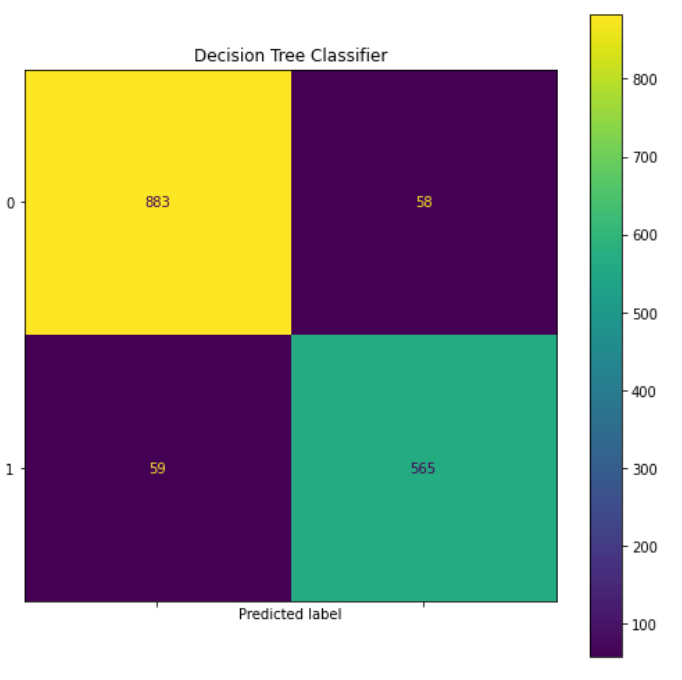
\includegraphics[width=0.25\linewidth]{confusion_tree.png}}
    \subfigure[]{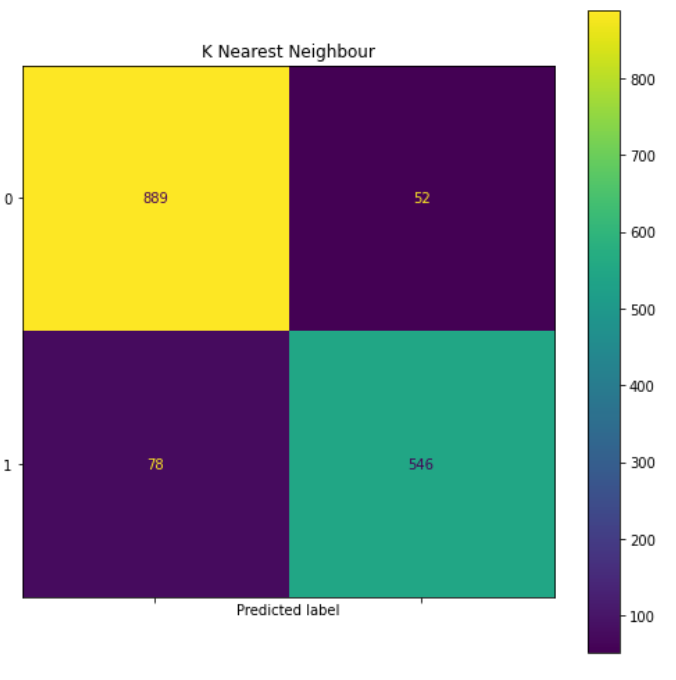
\includegraphics[width=0.25\linewidth]{confusion_knn.png}}
    \subfigure[]{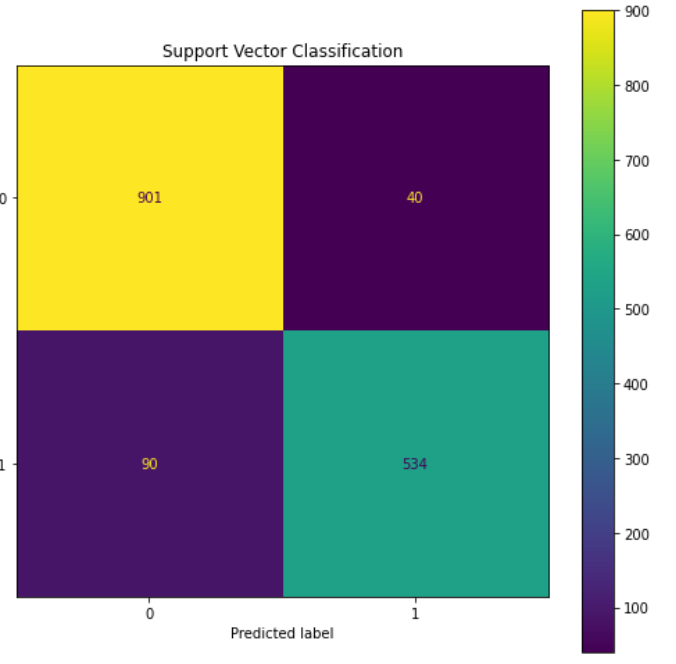
\includegraphics[width=0.25\linewidth]{confusion_svc.png}}
    \caption{}
\end{figure}


\clearpage
\section{Risultati}
In questa sezione vengono esposti i risultati raggiunti e come poter facilmente testare il funzionamento dell'algoritmo.

Tutti i parametri precedentemente utilizzati nei modelli sono stati scelti tramite una \textit{cross validation} a griglia. Sklearn dispone di una funzione chiamata \textit{GridSearchCV} che esegue la previsione con lo stesso algoritmo, ma con diversi parametri (precedentemente impostati dall'utente) e calcola la combinazione di parametri che \textbf{meglio si adatta al dataset}. Questi metodi hanno un tempo di esecuzione ed un costo computazionale solitamente alto, motivo per il quale una volta calcolati, sono stati salvati nel codice, o come si dice nel gergo informatico, sono \textit{"hard-coded"}.

I sample, prima di essere stati utilizzati negli agoritmi, sono stati normalizzati, per migliorare di gran lunga le previsioni. Vegnono rappresentate tre tabelle contenenti gli indicatori: la prima utilizzando i dati "crudi" senza nessun tipo di preprocessamento o miglioria dei parametri dei modelli; la seconda con i dati normalizzati; e la terza con sia il preprocessamento dei dati che i parametri discussi nel capitolo precedente.

Come si può velocemente notare dall'indicatore \textbf{f1-socre}, parametro maggiormente preso in considerazione, grazie a queste migliorie si riesce a perfezionare di quasi un 80\% l'algoritmo con previsioni peggiori, mentre di poco più di un 2\% negli alberi decisionali dove ha mantenuto le predizioni migliori.

\begin{figure}[h]
    \centering
    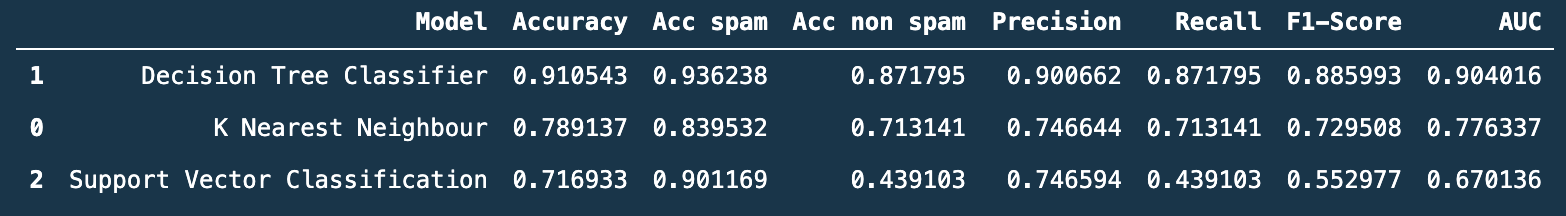
\includegraphics[width=1\linewidth]{results_nothing.png}
    \caption{Sample senza ottimizzazioni}
\end{figure}

\begin{figure}[h]
    \centering
    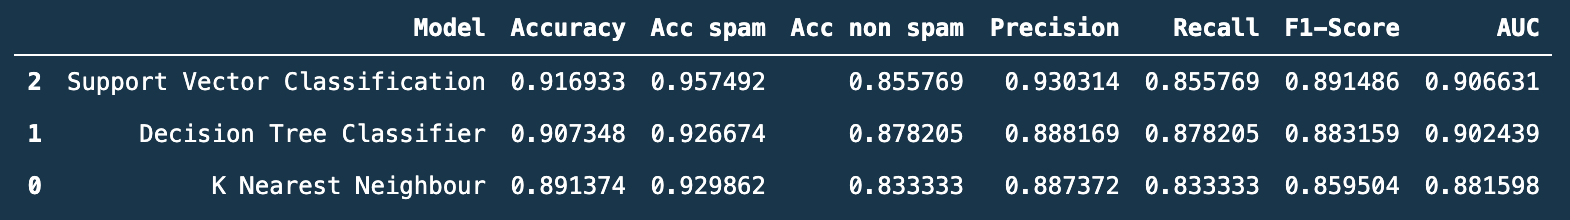
\includegraphics[width=1\linewidth]{results_scaler.png}
    \caption{Sample normalizzati}
\end{figure}

\begin{figure}[h]
    \centering
    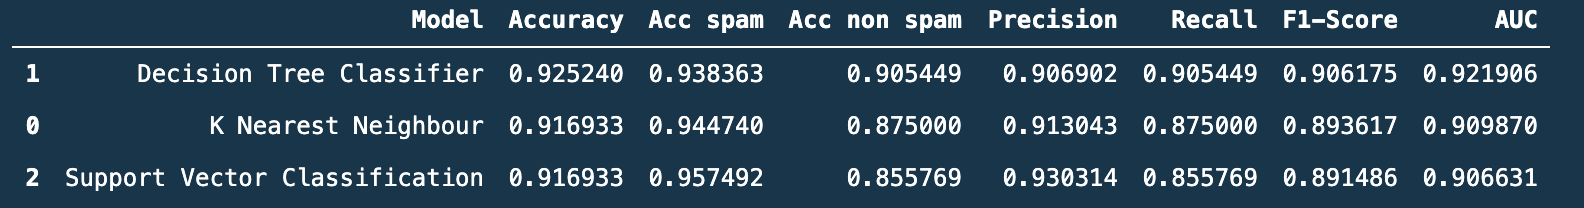
\includegraphics[width=1\linewidth]{results_optimized_all.png}
    \caption{Sample normalizzati e perfezionamento parametri}
\end{figure}

Da come è possibile notare dai grafici in figura 20 gli algoritmi attraverso queste ottimizzazioni hanno migliorato decisamente le previsioni della classe di appartenenza dell'email.
\break
\begin{figure}[H]
    \centering
    \subfigure[]{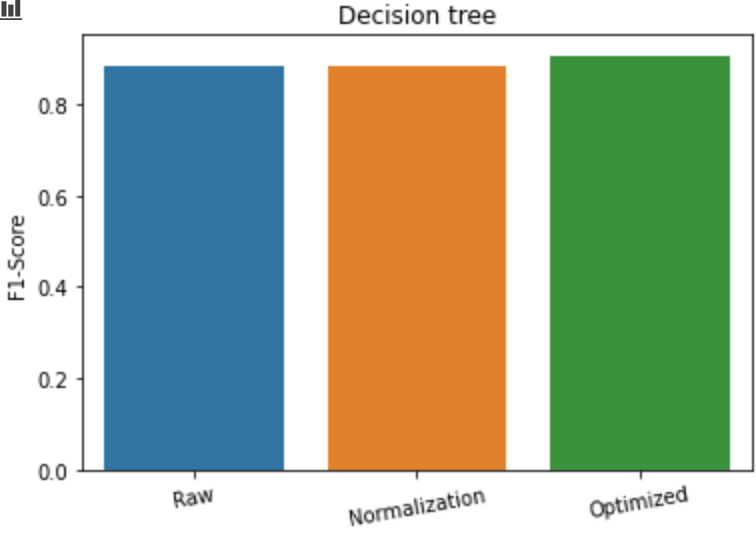
\includegraphics[width=0.3\linewidth]{decision_tree_results.png}}
    \subfigure[]{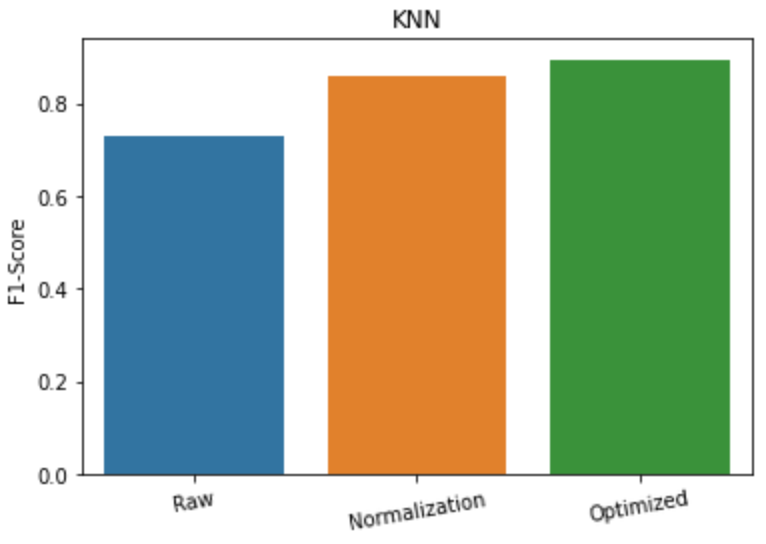
\includegraphics[width=0.3\linewidth]{knn_results.png}}
    \subfigure[]{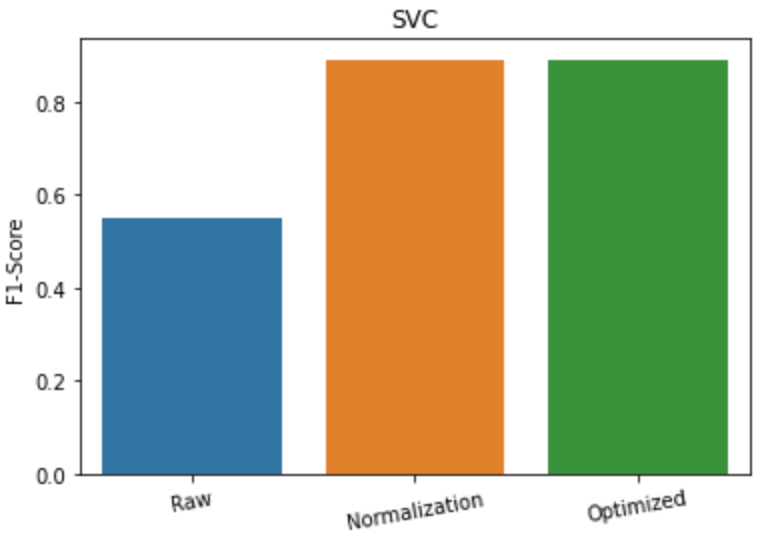
\includegraphics[width=0.3\linewidth]{svc_results.png}}
    \caption{}
\end{figure}


\section{API}
Attraverso l'utilizzo di Fast Api, una libreria python, si è implementata un'interfaccia grafica, facilmente raggiungibile tramite un browser, che permette di testare velocemente il corretto funzionamento del progetto.


\begin{figure}[h]
    \centering
    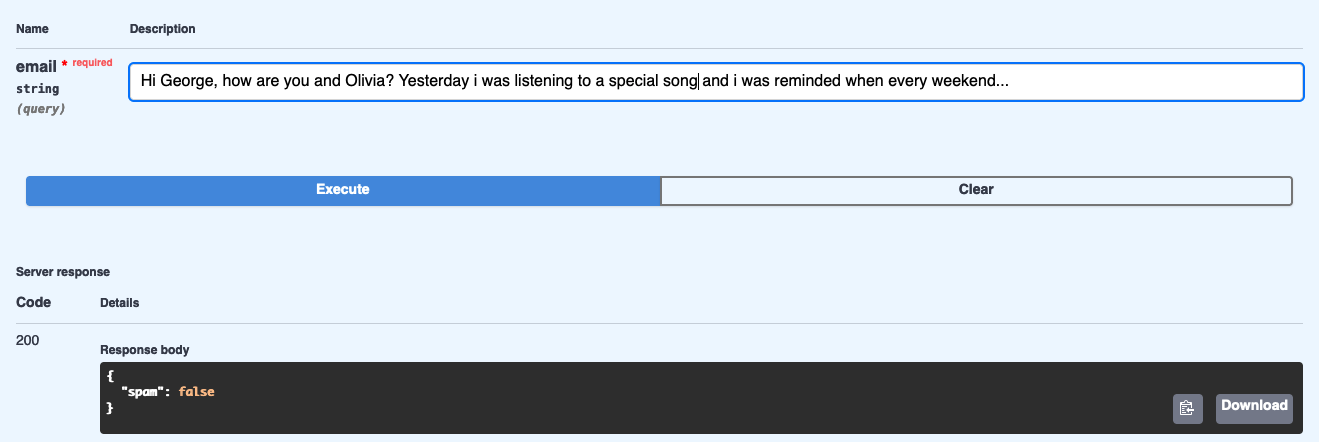
\includegraphics[width=1\columnwidth]{api_false.png}
    \caption{Non spam}
\end{figure}
\begin{figure}[h]
    \centering
    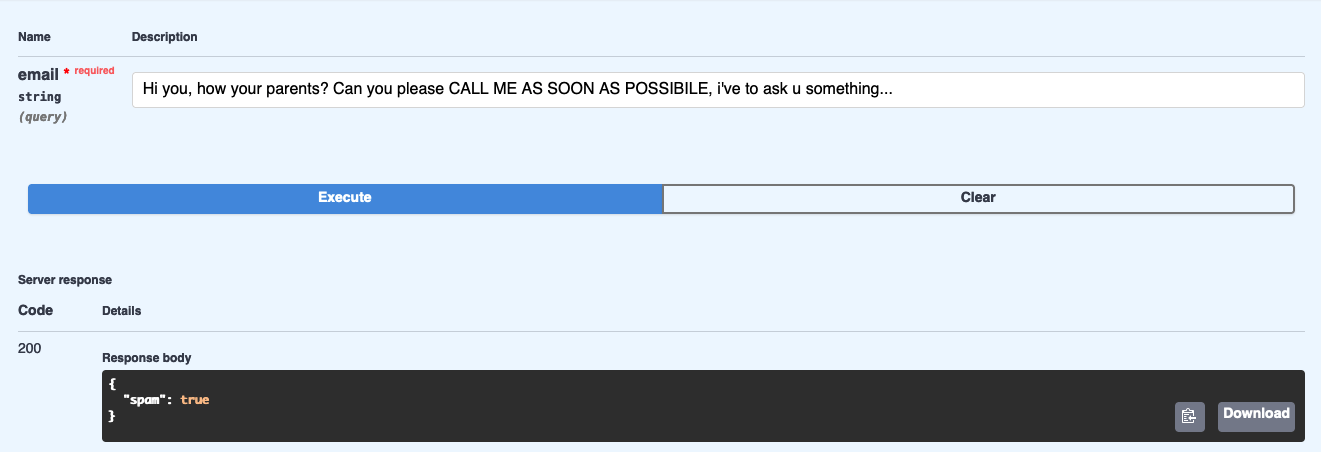
\includegraphics[width=1\columnwidth]{api_true.png}
    \caption{Spam}
\end{figure}

\begin{thebibliography}{9}
\addcontentsline{toc}{section}{References}
    \bibitem{}
        Silvia Cascianelli,
        \textit{Video lezioni e dispense di Machine Learning}.

    \bibitem{}
        Sito internet,
        \textit{it.wikipedia.org}

    \bibitem{}
        Sito internet,
        \textit{stackexchange.com}
    \bibitem{}
        Sito internet,
        \textit{stackoverflow.com}
    \bibitem{}
        Sito internet,
        \textit{scikit-learn.org}
    \bibitem{}
        Sito internet,
        \textit{blog.exsilio.com}
    \bibitem{}
        Sito internet,
        \textit{knowledgehut.com}
    \bibitem{}
        Sito internet,
        \textit{machinelearningmastery.com}
    \bibitem{}
        Sito internet,
        \textit{machinecurve.com}
    \bibitem{}
        Sito internet,
        \textit{lorenzogovoni.com}
    \bibitem{}
        Sito internet,
        \textit{towardsdatascience.com}

\end{thebibliography}

\end{document}
